\documentclass[11pt,a4paper]{article}
\usepackage{graphicx}
\usepackage{float}
\graphicspath{ {../scientific-experimentation-evaluation/} }
\usepackage{color}
\usepackage{listings}
\usepackage{hyperref}

\begin{document}
\title{\textbf{Scientific Experimentation and Evaluation}}
\author{Aaqib Parvez Mohammed \\ Chetan Sidnal\\ Mihir Patil \\ Sushma devaramani}
\date{\today}
\maketitle
\newpage
\tableofcontents
\newpage
\listoffigures
\newpage
\section{Experiment 1: Manual Motion Observation}
\textbf{Aim:} Manually measure the observable pose variation for three different constant velocity motions(Straight line, an arc to the left and an arc to the right) of LEGO NXT differential drive robot.

\subsection{\textbf{Setup}}
\begin{itemize}
\item The measurement system for the experiment includes a white sheet, a LEGO NXT differential drive robot, two pencils and a scale.
\item The \textbf{device under test(DUT)} is the LEGO NXT differential drive robot.
\item Clamp the sheet on a flat surface.
\item Construct a robot equipped with two pencils in the front, such that the start and end positions can be marked. This constitutes the measurement facility.
\item Install \textit{Lejos} OS on the robot.
\item Program the robot for it to run in three different constant velocity motions.
\end{itemize}

\begin{figure}[H]
\centering
  \centering
  \includegraphics[width=0.8\linewidth]{1}
  \caption{Side view}
  \label{fig:side}
\end{figure}

\begin{figure}[H]
\centering
  \centering
  \includegraphics[width=0.8\linewidth]{isometric}
  \caption{Isometric view}
  \label{fig:iso}
\end{figure}

\begin{figure}[H]
\centering
  \centering
  \includegraphics[width=0.8\linewidth]{Top}
  \caption{Top view}
  \label{fig:top}
\end{figure}

\begin{figure}[H]
\centering
  \centering
  \includegraphics[width=0.8\linewidth]{front}
  \caption{front view}
  \label{fig:front}
\end{figure}

\newpage
\subsection{\textbf{Procedure}}
\begin{itemize}
\item The experimental setup is prepared.
\item The starting position of the robot is marked with the help of the points drawn by the pencils.
\item The center of the line joining the two points is recorded which will be the starting position of the robot.
\item The robot is programmed to run in a straight line forward motion at a constant speed.
\item Once the robot stops, the center of the line joining the last points drawn by the pencils will be the stop position.
\item The \textbf{Measurand} i.e., the relative coordinates of the robot are measured by the difference in the coordinates of the starting position and the stopping position.
\item \textbf{Measurement System:} Our measurement system consists of robot placed on a cardboard sheet. Two pencils are attached in the front to mark the position. As the robot is moved, the path is traced on the sheet. After reaching the end position, the final pose is marked. The variation in the path is observed and the error in pose is measured.
\item The \textbf{Measurement result} i.e., the pose variation is obtained by finding the difference between the observed values and their mean.
\item Repeat the above experiment with a program to run the robot with constant angular and translational velocities for a fixed time period, such that it describes an arc to the left.
\item Repeat the above experiment with a program to run the robot with constant angular and translational velocities for a fixed time period, such that it describes an arc to the right.
\end{itemize}

\subsection{\textbf{Expected problems}}
\begin{itemize}
\item Parallax error.
\item Positional errors.
\item There might be slipping of wheels.
\item The tip of the pencils might break during the motion of the robot.
\item The pencils will have to be sharpened as the nibs might get blunt due to continuous drawing of lines which might result in measurement errors.
\end{itemize}

\subsection{\textbf{Expected performance}}
\begin{itemize}
\item The Rotation sensor measures the motor rotations with the accuracy of +/- one degree for one rotation(360 degree). Hence the accuracy in distance traveled for one rotation will be +/- 0.48mm. 
\item Reference: LEGO NXT: Features \& Limitations.
\item Assuming experiment distance = 704mm. Expected accuracy is $ \pm 2$ and expected precision 704mm is$ \pm 2$mm.
\end{itemize}

\subsubsection{Reasons}
\begin{itemize}
\item The slippage of the wheels may cause poor accuracy and precision.
\item The internal errors from the DUT may cause poor accuracy but the precision won't be affected significantly, since the DUT won't be changed while doing the measurement.
\end{itemize}

\subsection{Execution of the experiment:}
\begin{itemize}
\item The starting position of the robot was marked using two pencils which were placed on either side of the robot.
\item The same points were used as the starting points while repeating the experiment.
\item The position of the back wheel was also kept constant by drawing a line and using the same line as reference for future run of experiments.
\item The position of the back wheel impacted the outcome of the experiment as a small deviation from the reference line would result in a considerable deviation of the outcome.
\item The theta values were calculated by drawing a perpendicular to the line joining the two observed end points and calculating the angle using the formula $tan^{-1}(\frac{y}{x})$.
\item Lego NXT 2.0 software was used to program the robot with the following parameters.\\
No. of rotations = 4\\ 
Power = 40
\item {The battery voltage before the experiment = 8.2V. \\ The battery voltage after the experimmant = 4.2V.}
\item The observed data has been recorded in the ".csv" format.
\item There was no pre-processing of data required as no outliers were detected.
\item Graph has been plotted for all three motions. \\
Note : All x,y measurements are in inches
\subsubsection{Straight}
\begin{figure}[H]
\centering	
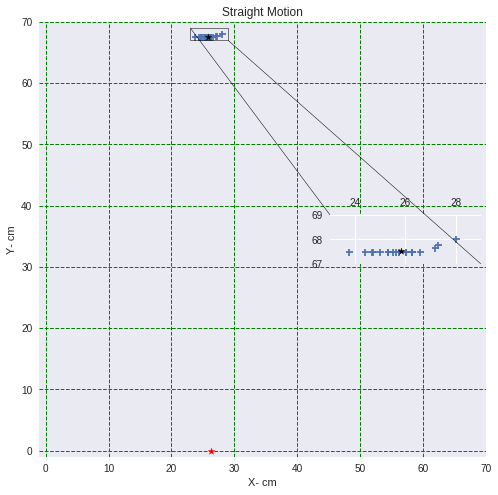
\includegraphics[width=1.2\linewidth]{Straight}
\label{fig:straight}
\caption{20 iteration of moving straight}
\end{figure}

\newpage
\textbf{Fitting the distribution for the obtained data: \\ (X, Y) points for straight line}
\begin{figure}[H]
\centering	
\includegraphics[width=0.8\linewidth]{straightG}
\label{fig:straightG}
\caption{Density plot of (X,Y) for straight line motion}
\end{figure}

In the above graph, it can be observed that 'X' points fit a gaussian distribution, whereas 'Y' points does not fit any distribution, since they are mostly precise and accurate.
%   \begin{figure}[H]
% 	\centering	
% 		\includegraphics[width=1.0\linewidth]{bplot_straight}
% 		\label{fig:sub1}
% 	\caption{\color{blue}Box plot for (X, Y) points in straight line}
%   \end{figure}
\begin{itemize}
\item $ Range (x,y) =([23.77-28.01],[67.50-68.01]) $
\item $ Mean (x, y) = 25.81,67.54$
\item $ \sigma (x, y)= 1.01, 0.12 $
\item $ Accuracy (x,y) = x \pm0.9  , y \pm0.1 $  
\end{itemize}

\subsubsection{Right}
\begin{figure}[H]
\centering	
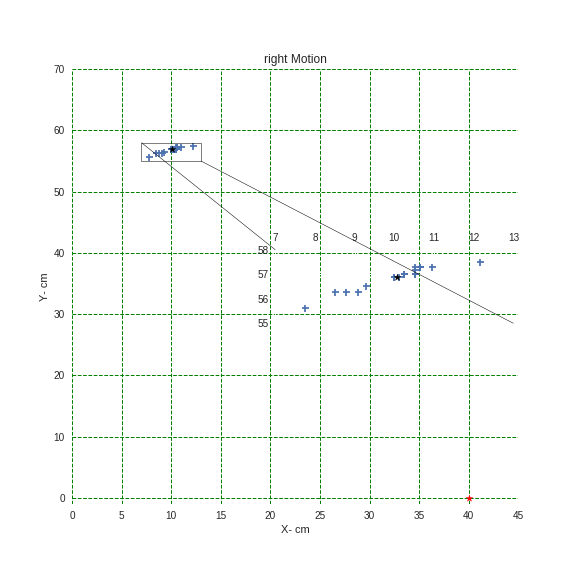
\includegraphics[width=1.2\linewidth]{right_i}
\label{fig:right}
\caption{20 observations of right arc motion}
\end{figure}

\begin{figure}[H]
\centering	
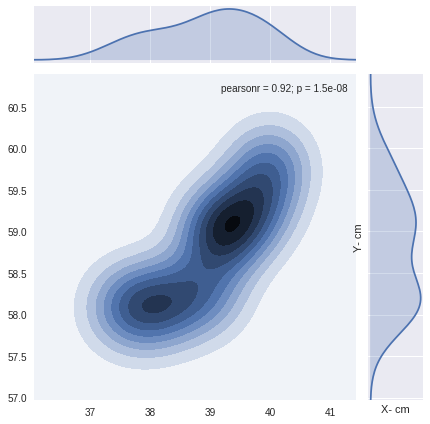
\includegraphics[width=0.8\linewidth]{rightG}
\label{fig:sub1}
\caption{Density plot of (X, Y) points for right arc motion}
\end{figure}

In the above plot it can be observed that the distribution of X and Y positions for right arc motion is gaussian.
%   \begin{figure}[H]
% 	\centering	
% 		\includegraphics[width=1.0\linewidth]{dist_plot}
% 		\label{fig:sub1}
% 	\caption{\color{blue}20 iteration distribution plot}
%   \end{figure}

\begin{itemize}
\item $ Range (x,y) =([37.50-40.00],[58.01-59.78])  $
\item $ Mean (x, y) = 38.95,58.77$
\item $ Accuracy (x,y) = x \pm0.5 , y \pm0.5  $ 
\item $ \sigma (x, y)= 0.81, 0.61 $
\item $ Mean(\theta) = 40.58 degree$
\item $ Accuracy (\theta)= \theta \pm5  deg $
\item $ \sigma = 1.09 deg$
\item $ range (\theta) = 38.83 - 43.33 $
\end{itemize}

\subsubsection{Left}
\begin{figure}[H]
\centering	
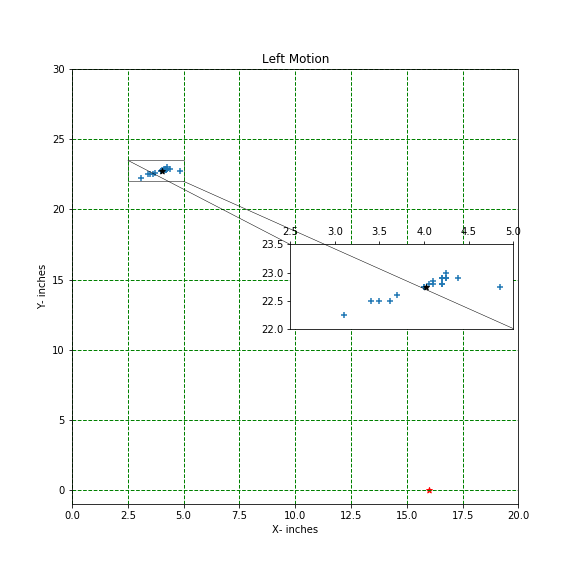
\includegraphics[width=1.2\linewidth]{left_i}
\label{fig:sub1}
\caption{20 iteration of moving left}
\end{figure}

\begin{figure}[H]
\centering	
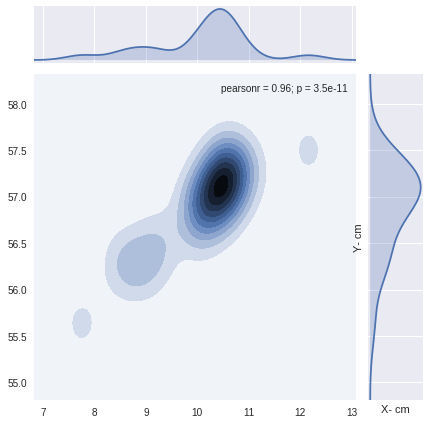
\includegraphics[width=1.0\linewidth]{leftG}
\label{fig:sub1}
\caption{Density plot of (X, Y) for moving left}
\end{figure}

In the above figure it can be observed that the (X, Y) points obtained for left arc motion fit a gaussian distribution.
%   \begin{figure}[H]
% 	\centering	
% 		\includegraphics[width=1.0\linewidth]{bplot_left}
% 		\label{fig:sub1}
% 	\caption{\color{blue}Box plot for 20 iterations of left arc motion}
%   \end{figure}
\begin{itemize}
\item $ Range (x,y) =([7.75-12.16],[55.63-57.50])  $
\item $ Mean (x, y) = 10.05,56.89$
\item $ Accuracy (x,y) = x \pm0.5 , y \pm0.5  $ 
\item $ \sigma (x, y)= 0.97, 0.47 $
\item $ Mean(\theta) = 45.71 degree$
\item $ Accuracy (\theta)= \theta 7\pm  deg $
\item $ \sigma = 1.32 deg$
\item $ range (\theta) = 43.18 - 48.27 $
\end{itemize}
\end{itemize}

% \subsection{Straight Motion}
% \begin{table}
% \centering
% \pgfplotstabletypeset[dec sep align,
%    fixed zerofill,
%    precision=4,
%    col sep=space]{leftT.csv}
% \end{table}

% \subsection{Right Motion}

% \subsection{Left Motion}

\textbf{Boxplots}
\begin{figure}[H]
\centering
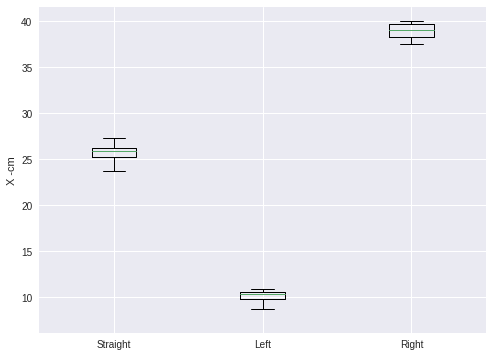
\includegraphics[width=1.0\linewidth]{boxplot-x}
\label{fig:box-x}
\caption{Box plot of X-values for straight line motion, left and right turn}
\end{figure}

\begin{figure}[H]
\centering	
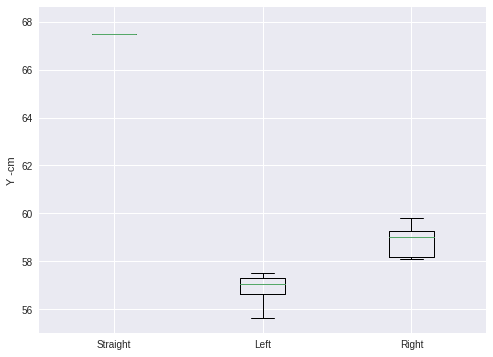
\includegraphics[width=1.0\linewidth]{boxplot-y}
\label{fig:box-y}
\caption{Box plot of Y-values for straight line motion, left and right turn}
\end{figure}

\begin{itemize}
\item 2.3 The chi-square test indicates that the observed data is a normal distribution.
\begin{lstlisting}[language=Python]
In [9]: ks , p = stats.normaltest(straight_xy)
		alpha = 1e-3
        # null hypothesis: x comes from normal distribution
		if p.all() < alpha: 
			print("The null hypothesis can be rejected")
		else:
			print("The null hypothesis cannot be rejected")
            
[Out]: The null hypothesis cannot be rejected

In [10]: ks , p = stats.normaltest(right_xy)
		alpha = 1e-3
		if p.all() < alpha: 
			print("The null hypothesis can be rejected")
		else:
			print("The null hypothesis cannot be rejected")
[Out]: The null hypothesis cannot be rejected

In [11]: ks , p = stats.normaltest(left_xy)
		alpha = 1e-3
		if p.all() < alpha: 
			print("The null hypothesis can be rejected")
		else:
			print("The null hypothesis cannot be rejected")
[Out]: The null hypothesis cannot be rejected
\end{lstlisting}

\item Deliverable 2.2: The functions used for plotting are from the seaborn library and use a kernel density method to obtain a 2-D density plot of the x and y coordinates. 
\item Deliverable 2.5:
\subsection{Straight}
\begin{itemize}
\item In the case of straight line motion the readings obtained for Y coordinates appear to be both precise and accurate, whereas the X coordinates appear to be precise but not very accurate.
\end{itemize} 
\subsection{Right}
\begin{itemize}
\item The readings obtained for Y coordinates appear to be both highly precise and accurate, whereas the X coordinates appear to be precise but not very accurate.
\end{itemize}
\subsection{Left}
\begin{itemize}
\item The readings obtained for X coordinates appear to have low precision and accuracy, whereas the Y coordinates appear to be precise with a low accuracy.
\end{itemize}
\end{itemize}
\section{Appendix}
\subsection{Softwares used}
\begin{itemize}
\item Python 2.7
\item Jupyter Notebook
\end{itemize}

\subsection{Packages used}
\begin{itemize}
\item Matplotlib
\item Numpy
\item Scipy
\item Seaborn
\item Pylab
\end{itemize}

\subsection{Tools used}
\begin{itemize}
\item Onscreen ruler is used to mark scale on the sheet (metrics in inches)
\item \url{https://www.piliapp.com/actual-size/inch-ruler/}
\begin{figure}[H]
\centering	
\includegraphics[width=0.4\linewidth]{screenshot}
\label{fig:sub1}
\caption{Online ruler}
\end{figure}

\begin{figure}[H]
\centering	
\includegraphics[width=0.7\linewidth]{measure}
\label{fig:sub1}
\caption{Marking scale on the sheet using onscreen ruler}
\end{figure}

\end{itemize}
\end{document}
